\chapter{Theoretical Framework}

Tyter. 

\section{Galaxy Clusters}
 
Glas.

dwarf stars contribute very little to the integrated light from an old stellar population (Smith 2015)

Galaxy clusters contain a population of stars gravitationally unbound to individual galaxies, yet still bound to the clusters overall gravitational potential, created by the stripping of stars from galaxies during interactions and mergers

\begin{figure}[H]
\centering
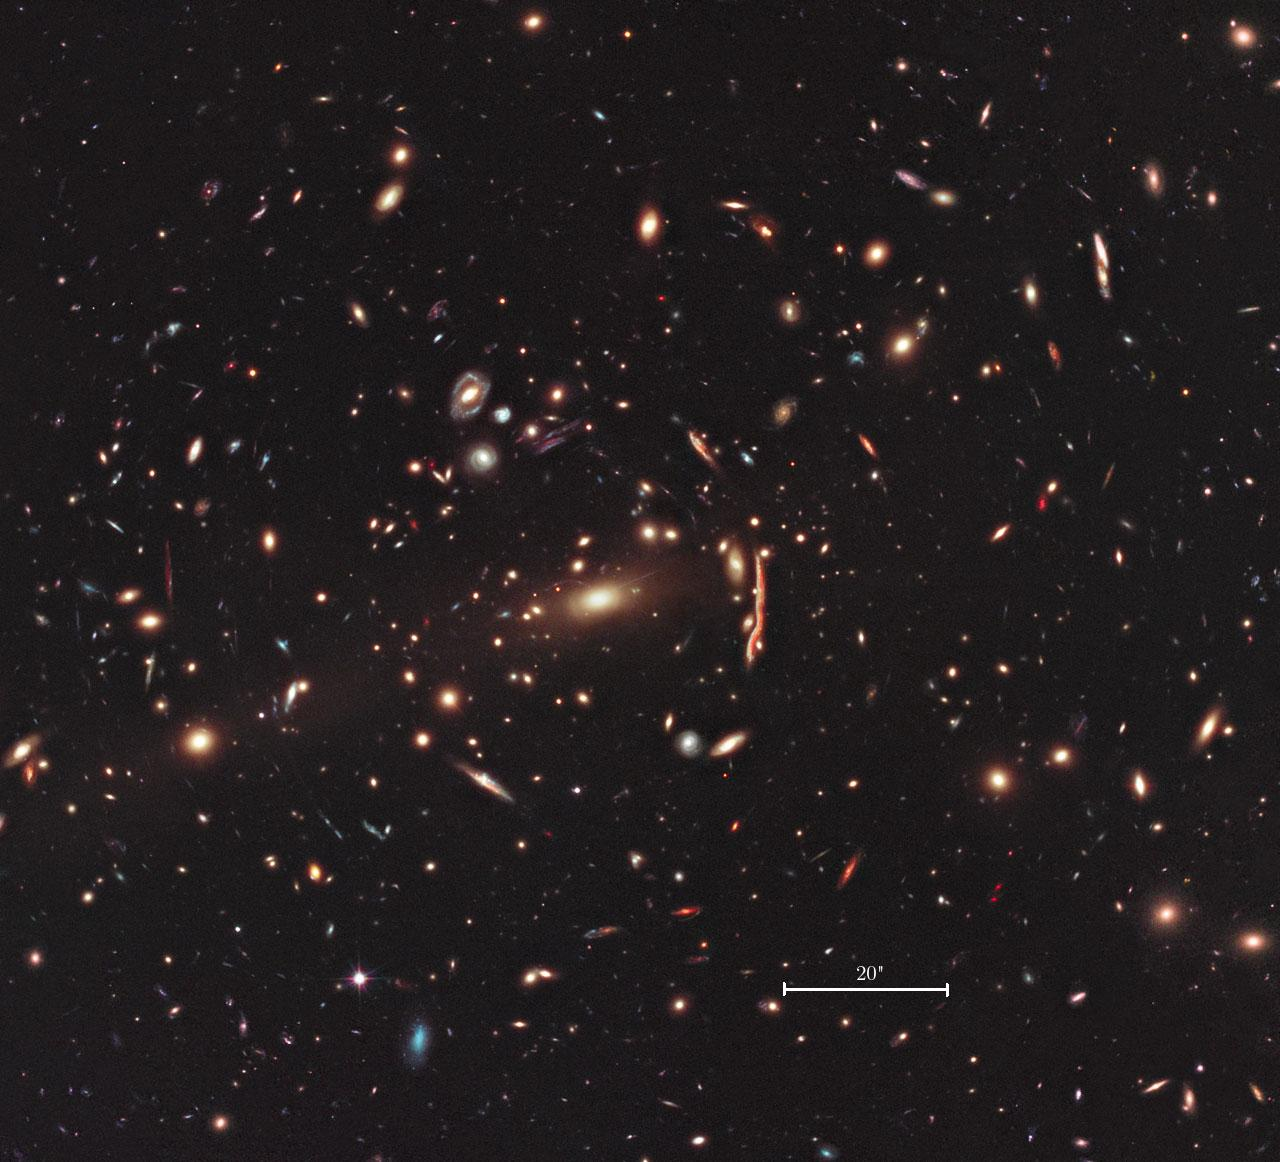
\includegraphics[width=12cm]{images/GC.jpg}
\caption[M]{G}
\end{figure}

Quoted (need to change this):The image of galaxy cluster MACS J1206.2-0847 (or MACS 1206) is part of a broad survey with NASA Hubble Space Telescope.The distorted shapes in the cluster are distant galaxies from which the light is bent by the gravitational pull of an invisible material called dark matter within the cluster of galaxies. This cluster is an early target in a survey that will allow astronomers to construct the most detailed dark matter maps of more galaxy clusters than ever before.These maps are being used to test previous, but surprising, results that suggest that dark matter is more densely packed inside clusters than some models predict. This might mean that galaxy cluster assembly began earlier than commonly thought.

Scientists are planning to observe a total of 25 galaxy clusters under a project called CLASH (Cluster Lensing and Supernova survey with Hubble).One of the first objects observed for the new census is the galaxy cluster MACS J1206.2-0847. This conglomeration of galaxies is one of the most massive structures in the universe, and its gigantic gravitational pull causes stunning gravitational lensing. MACS 1206 lies 4 billion light-years from Earth. In addition to curving of light, gravitational lensing often produces double images of the same galaxy. In the new observation of cluster MACS J1206.2-0847, astronomers counted 47 multiple images of 12 newly identified galaxies.The era when the first clusters formed is not precisely known, but is estimated to be at least 9 billion years ago and possibly as far back as 12 billion years ago. If most of the clusters in the CLASH survey are found to have excessively high accumulations of dark matter in their central cores, then it may yield new clues to the early stages in the origin of structure in the universe.


\section{Gravitational Lensing}

At small radii, stars dominate the lensing mass, so that lensing provides a direct probe of the stellar mas to light ratio, with only small corrections needed for darl matter.

In the paper of Russell Smith (a giant elliptical galaxy with a lightweight initial mass funciton) they find a stellar mass to light ratio of 3.01 plus minus 0.25

Modelling the lensing configuration provides the total projection mass within an aperture.

NFW profile for dark matter that is basically the dynamical mass of the cluster

let's take the case of ABELL1068, it's magnitude in U is 21.94, in I is 18.46, in g is 20.09, in r is 19.5, also $M_{200}=4.3\times 10^{14}M_{\odot}$

The bolometric luminosity of Abell1068 is $10^44$erg/s that in solar luminosities is $2.599\times 10^{10} L_sol$, this gives an effective brightness of $10^{6}M_{\odot}/kpc^2$.

the distance to the galaxy is 591.42857 Mpc	

salpeter mass function is $n(M)\propto M^{-2.3}$  

de Vaucouleurs law for the surface brightness distribution in giant elliptical galaxies is:

\begin{equation}
I(R)=I_{e}e^{-b\left[\left(R/R_{e}\right)^{1/4}-1\right]}
\end{equation}

where $b=7.67$ and $I_{e}$ is the effective brightness which is basically the brightness at the effective radius $R_{e}$

From the paper of Lokas and Mamon, for constant mass-light-ratio we have $\Sigma_{M}(R)=\Gamma I(R)$ where I is the surface brightness.

the NFW density profile is 

\begin{equation}
\rho(r)=\frac{\delta_{c}\rho_{c}}{(r/r_{s})(1+r/r_{s})^{2}}
\end{equation}

where the characteristic overdensity is:

\begin{equation}
\delta_{c}=\frac{200}{3}\frac{c^{3}}{\ln{(1+c)}-c/(1+c)}
\end{equation}

from Munoz cuartas et. al. we see that the concentration parameter depends on the mass and the redshift as we see in the following plot:

\begin{figure}[H]
\centering
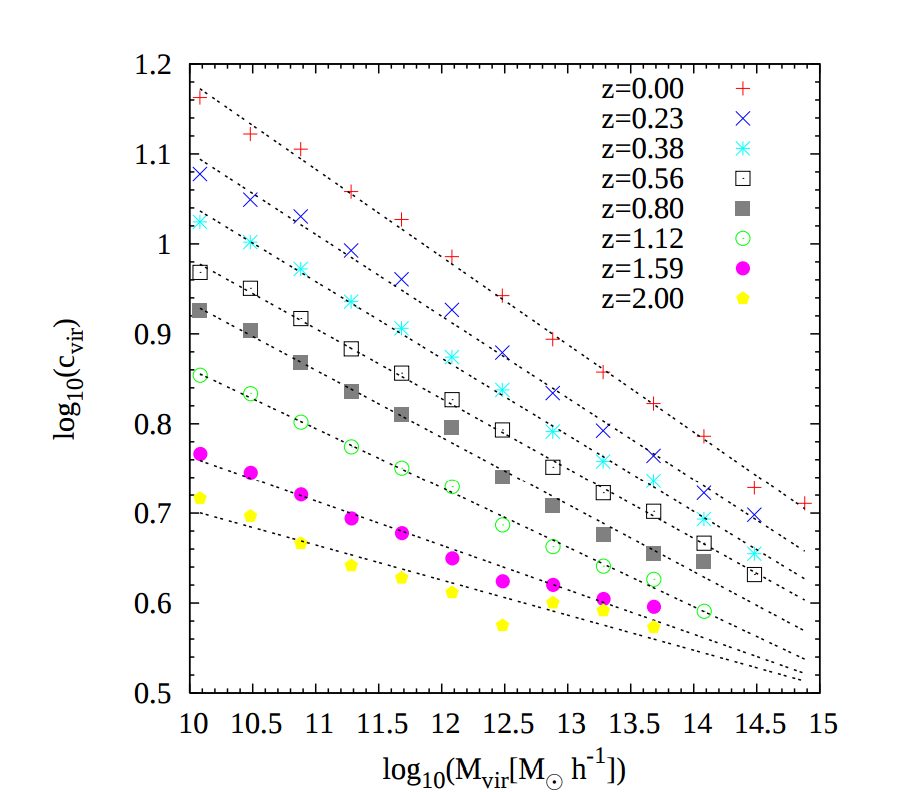
\includegraphics[width=12cm]{images/juank.png}
\caption[M]{G}
\end{figure}


$c=r_{200}/r_{s}$

The concentration parameter c is strongly correlated with Hubble type, c=2.6 separating early from late-type galaxies. Those galaxies with concentration incides c>2.6 are early-type galaxies reflecting the fact that the light is more concentrated towards their centres

From Dutton and Maccio 2014 we get the following image for the concentration parameter:

\begin{figure}[H]
\centering
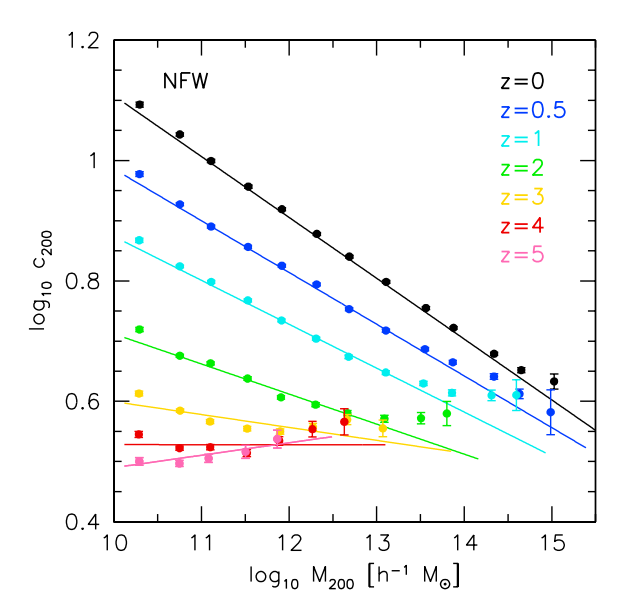
\includegraphics[width=12cm]{images/dutton.png}
\caption[M]{G}
\end{figure}


The surface mass density is given by:

\begin{equation}
\Sigma_{\text{NFW}}(x) = \left\lbrace
\begin{array}{lll}
\frac{2r_{s}\delta_{c}\rho_{c}}{\left(x^{2}-1\right)}\left[1-\frac{2}{\sqrt{1-x^{2}}}\arctanh\sqrt{\frac{1-x}{1+x}}\right](x<1) & (x<1)\\\\
\frac{2r_{s}\delta_{c}\rho_{c}}{3}(x=1) & (x=1)\\\\
\frac{2r_{s}\delta_{c}\rho_{c}}{\left(x^{2}-1\right)}\left[1-\frac{2}{\sqrt{x^{2}-1}}\arctan\sqrt{\frac{x-1}{1+x}}\right](x<1) & (x>1)
\end{array}
\right.
\end{equation} 

then the concentration parameter for ABELL1068 is about 7.9 supposing a mass of the galaxy of $10^{12.5}M_{\odot}$

so from the critical density:

\begin{equation}
\rho_{c}=\frac{3H^2(z)}{8\pi G}
\end{equation}

the critical density would be: $2\times 10^{-26}$ in SI units so in Msol/pc3 it is $2.9\times 10^{-7}$

$H(z)=H_{0}(1+\Omega z)^{3/2}$

the Hubble parameter at z=0.138 is H(z)=85.6

delta c is 25315 (dimensionless)

The characteristic radius is given by $r_{1/2}=1.34R_{e}$

Here the surface mass density for both the stellar content and the NFW profile:

\begin{figure}[H]
\centering
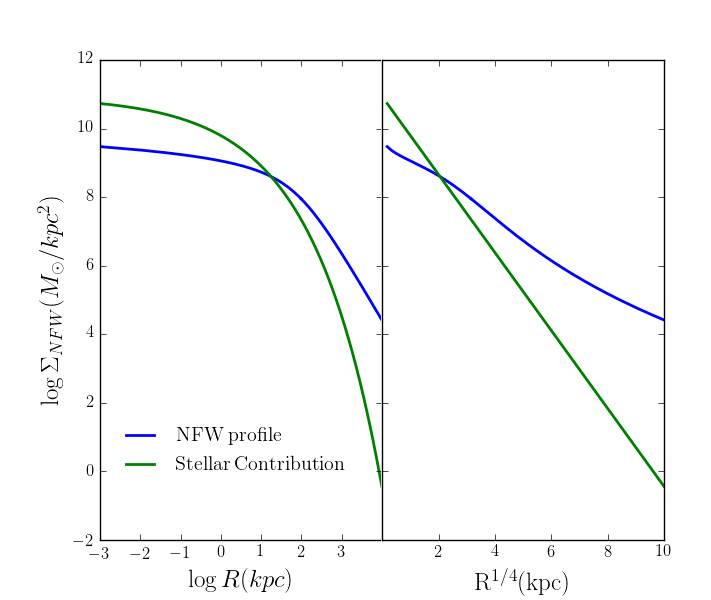
\includegraphics[width=12cm]{images/Surface_mass_density_log.png}
\caption[M]{G}
\end{figure}

But we are more interested in the enclosed mass which can be done by integrating the surface mass density:

\begin{equation}
M(R)=\int_{0}^{R}2\pi R\Sigma(R)dR
\end{equation}

And the plot for the enclosed mass is:

\begin{figure}[H]
\centering
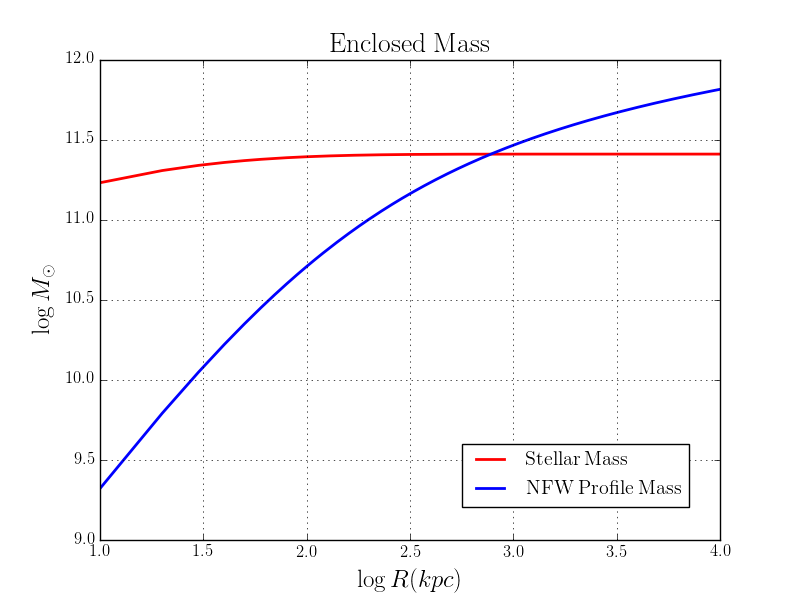
\includegraphics[width=12cm]{images/Enclosed Mass.png}
\caption[M]{G}
\end{figure}

The radial dependence on the shear is:

\begin{equation}
\gamma_{\text{NFW}}(x) = \left\lbrace
\begin{array}{lll}
\frac{r_{s}\delta_{c}\rho_{c}}{\Sigma_c}g_{<}(x) & (x<1)\\\\
\frac{r_{s}\delta_{c}\rho_{c}}{\Sigma_c}\left[\frac{10}{3}+4 \ln \left(\frac{1}{2}\right)\right] & (x=1)\\\\
\frac{r_{s}\delta_{c}\rho_{c}}{\Sigma_c}g_{>}(x) & (x>1)
\end{array}
\right.
\end{equation} 

where: 

\begin{equation}
g_{<}(x)=\frac{8 \arctanh \sqrt{\frac{1-x}{1+x}}}{x^{2}\sqrt{1-x^{2}}}+\frac{4}{x^{2}} \ln \left(\frac{x}{2}\right)-\frac{2}{\left(x^{2}-1\right)}+\frac{4 \arctanh \sqrt{\frac{1-x}{1+x}}}{\left(x^{2}-1\right)\left(1-x^{2}\right)^{1/2}}
\end{equation}

\begin{equation}
g_{<}(x)=\frac{8 \arctan \sqrt{\frac{x-1}{1+x}}}{x^{2}\sqrt{x^{2}-1}}+\frac{4}{x^{2}}\ln \left(\frac{x}{2}\right)-\frac{2}{\left(x^{2}-1\right)}+\frac{4 \arctan \sqrt{\frac{x-1}{1+x}}}{\left(x^{2}-1\right){}^{3/2}}
\end{equation} 

and with teh critical surface mass density:

\begin{equation}
\Sigma_{c}\equiv\frac{c^{2}}{4\pi G}\frac{D_{s}}{D_{d}D_{ds}}
\end{equation}

these equations come from the paper Wright and Brainerd 1999

the plot of the radial dependence on the radius is:

\begin{figure}[H]
\centering
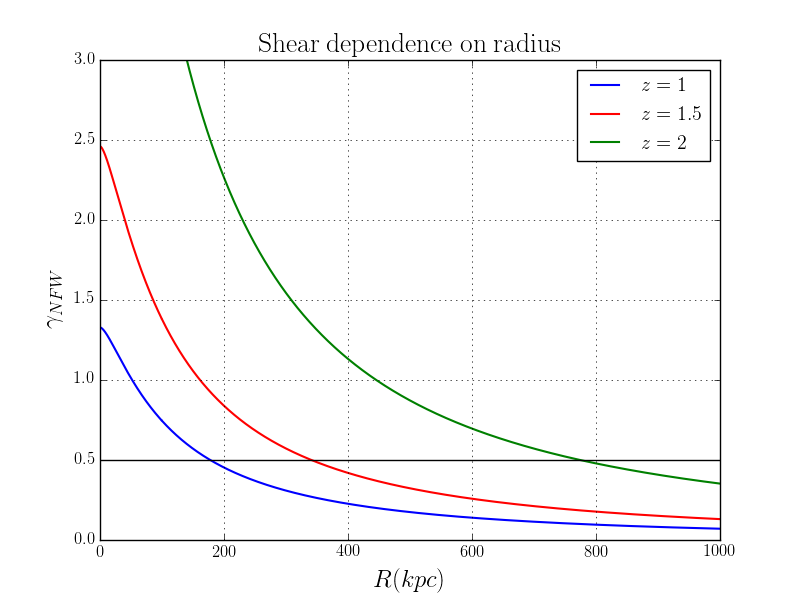
\includegraphics[width=12cm]{images/Shear dependence on radius.png}
\caption[M]{G}
\end{figure}


\section{IMF in BCGs}

For stars, measurements of the luminosity function can be
used to derive the Initial Mass Function (IMF).
For galaxies, this is more difficult because Mass to light ratio (M/L) of the stellar population
depends upon the star formation history of
the galaxy.

bulges have heavier IMFs than disks

Several recent studies have presented evidence for "heavyweight" IMFs in giant ellipticals, with a mass-to-light-ratio twice that of a Milky Way like IMF.



 
 